%!TEX root = main.tex
\setcounter{chapter}{2}
\setcounter{section}{5}
\setcounter{theorem}{0}
\setcounter{equation}{0}

\lectureheader{161}{Calculus I}{Limit practice}{\textit{Thomas' Calculus} \thesection}

\begin{definition}[Continuity at a point]\,
\begin{itemize}
\item We say that $f$ is \textbf{continuous} at $x=c$ if $\DS\lim_{x\to c}f(x) = f(c)$.
\item If $f$ is not continuous at $x=c$, then we say that $f$ is \textbf{discontinuous} at $x=c$.
\item We say that $f$ is \textbf{right-continuous} at $x=c$ if $\DS\lim_{x\to c^+}f(x) = f(c)$.
\item We say that $f$ is \textbf{left-continuous} at $x=c$ if $\DS\lim_{x\to c^-}f(x) = f(c)$.
\end{itemize}
\end{definition}

\begin{remark}
The definition of continuous is saying 3 things in that one equation.
\begin{enumerate}
\item $f(c)$ is defined, i.e., $c\in\dom(f)$.
\item $\DS\lim_{x\to c}f(x)$ exists.
\item The function value and the limit at $x=c$ agree.
\end{enumerate}
\end{remark}

\begin{example}
Determine where the function below is continuous/discontinuous.\\
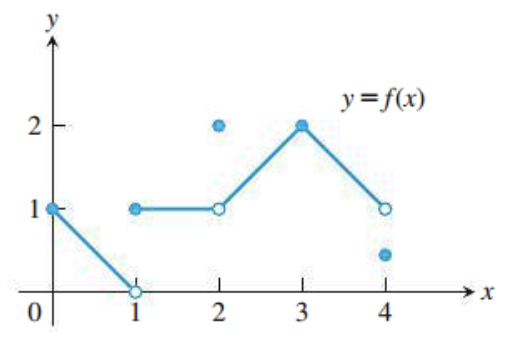
\includegraphics[width=3in]{img/continuity-ex1}
\end{example}

\newpage

\begin{definition}[Discontinuity types]\,
\begin{itemize}
\item We say that $f$ has a \textbf{removable discontinuity at $x=c$} if
\begin{enumerate}
\item $\DS\lim_{x\to c}f(x)$ exists, but
\item $f(c)$ is undefined or $\DS\lim_{x\to c}f(x)\ne f(c)$.
\end{enumerate}
\item We say that $f$ has a \textbf{jump discontinuity at $x=c$} if
\begin{enumerate}
\item $\DS\lim_{x\to c^+}f(x)$ and $\DS\lim_{x\to c^-}f(x)$ both exist, but
\item $\DS\lim_{x\to c^+}f(x)\ne\DS\lim_{x\to c^-}f(x)$
\end{enumerate}
\item We say that $f$ has an \textbf{infinite discontinuity at $x=c$} if 
\begin{equation*}
\DS\lim_{x\to c^+}f(x)=\pm\infty\text{ or }\DS\lim_{x\to c^-}f(x)=\pm\infty.
\end{equation*}
\item We say that $f$ has an \textbf{oscillating discontinuity at $x=c$} if 
$f(x)$ gets arbitrarily close to 2 or more values as $x\to c^{\pm}$.
\end{itemize}
\end{definition}

\begin{example}
Give an example of each type of discontinuity.
\end{example}

\newpage

\begin{definition}[Continuity on an interval]\,
\begin{itemize}
\item We say $f$ is \textbf{continuous on the open interval $(a,b)$} if it is continuous at every point $c\in (a,b)$.
\item We say $f$ is \textbf{continuous on the closed interval $[a,b]$} if
\begin{enumerate}
\item it is continuous at every point $c\in (a,b)$,
\item it is right-continuous at $a$, and
\item it is left-continuous at $b$.
\end{enumerate}
\end{itemize}
\end{definition}

\begin{definition}[Continuous functions]\,
Let $f$ be a function with domain $D$.
\begin{enumerate}
\item We say that $f$ is a \textbf{continuous function} if it is continuous at every point in $D$.
\item We say that $f$ is a \textbf{discontinuous function} if it is discontinuous at one or more points in $D$.
\end{enumerate}
\end{definition}
\begin{remark}
A function always has a specified domain. To change the domain is to change the function, and hence its continuity property may change as well.
\end{remark}

\begin{example}
Discuss the continuity properties of $f(x)=1/x$ on its natural domain versus an interval $I$ containing $x=0$.
\end{example}

\newpage

\begin{theorem}\,
The following types of functions are continuous on their natural domains:
\begin{enumerate}
\item polynomial functions,
\item rational functions,
\item algebraic functions (i.e., roots of rational functions),
\item trigonometric functions.
\end{enumerate}
\end{theorem}

\begin{remark}
The above theorem isn't saying that these functions do not have discontinuities.
It is only claiming that they are continuous everywhere that they are defined.
\end{remark}


\begin{example}
The function $y=\sec x$ has infinite discontinuities at every odd multiple of $\frac{\pi}{2}$.
However, 
\begin{equation*}
\dom(\sec) = \left\{x: x\ne (2n+1)\frac{\pi}{2}, n\in\Z\right\}.
\end{equation*}
\begin{center}
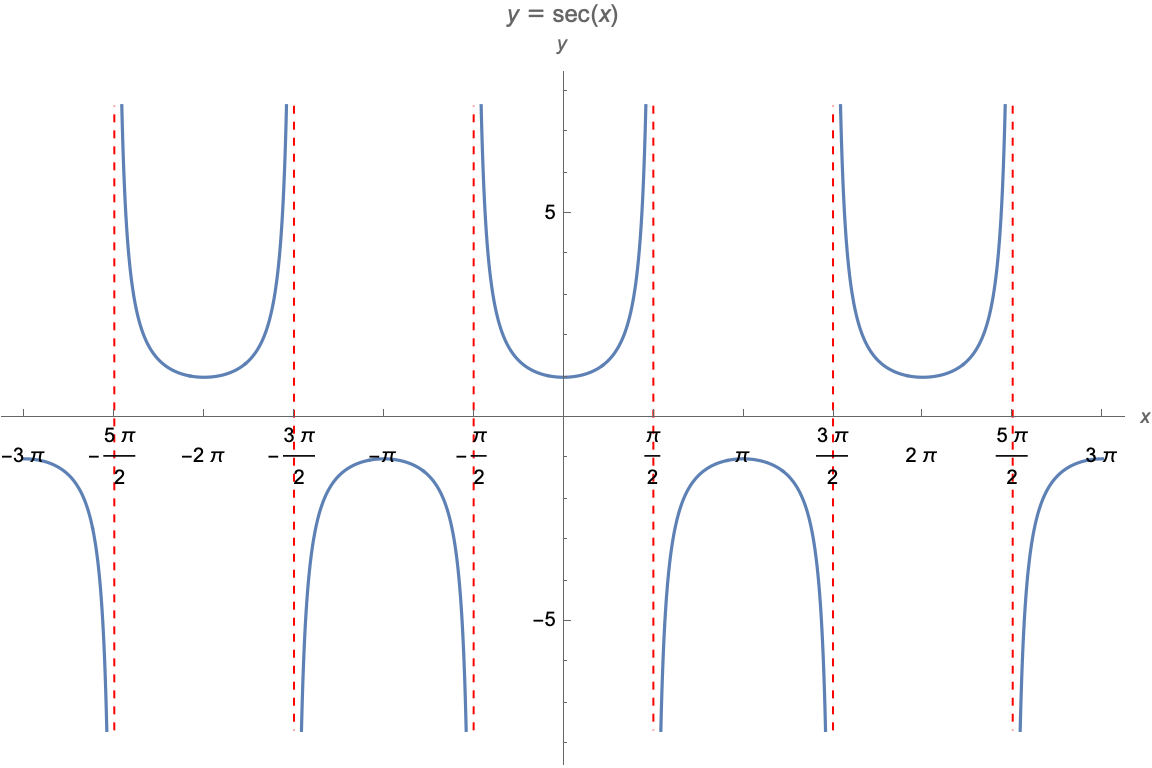
\includegraphics[width=4in]{img/sec}
\end{center}
\end{example}

\vfill

\begin{theorem}
If $f$ and $g$ are both continuous at $x=c$, then the following are also continuous at $x=c$:
\begin{enumerate}
\item $f\pm g$,
\item $f\cdot g$,
\item $f/g$ (provided $g(c)\ne 0$).
\end{enumerate}
\end{theorem}

\begin{theorem}
If $f$ is continuous at $c$ and $g$ is continuous at $f(c)$, then $g\circ f$ is continuous at $c$.
\end{theorem}

\newpage

\begin{example}
Show that the following are continuous on their natural domains.
\begin{enumerate}
\item $y=\sqrt{x^2-2x-5}$
\vfill
\item $y=\DS\frac{x^{2/3}}{1+x^4}$
\vfill
\end{enumerate}
\end{example}

\newpage

\begin{example}
Show that the following are continuous on their natural domains.
\begin{enumerate}
\item $y=\DS\left|\frac{x-2}{x^2-2}\right|$
\vfill
\item $y=\DS\left|\frac{x\sin x}{x^2+2}\right|$
\vfill
\end{enumerate}
\end{example}

\newpage

\begin{definition}[Continuous extension]
If $f$ has a removable discontinuity at $x=c$, then
\begin{equation*}
F(x) = \begin{cases}
f(x) & \text{if }x\ne c,\\
\DS\lim_{x\to c}f(x) & \text{if } x=c
\end{cases}
\end{equation*}
is called the \textbf{continuous extension of $f$ to $x=c$}.
\end{definition}

\begin{example}
Show that the function $f(x)=\DS\frac{x^2+x-6}{x^2-4}$ has a continuous extension to $x=2$.
\end{example}

\vfill

\begin{example}
Show that the function $f(x)=\DS\frac{\sin x}{x}$ has a continuous extension to $x=0$.
The continuous extension is known as $\sinc x$.
\end{example}

\vfill



\newpage

\begin{theorem}[Intermediate value theorem]
If $f$ is continuous on $[a,b]$, and if $y_0$ is between $f(a)$ and $f(b)$, then there is a $c\in [a,b]$ so that $f(c)=y_0$.
\end{theorem}
\begin{center}
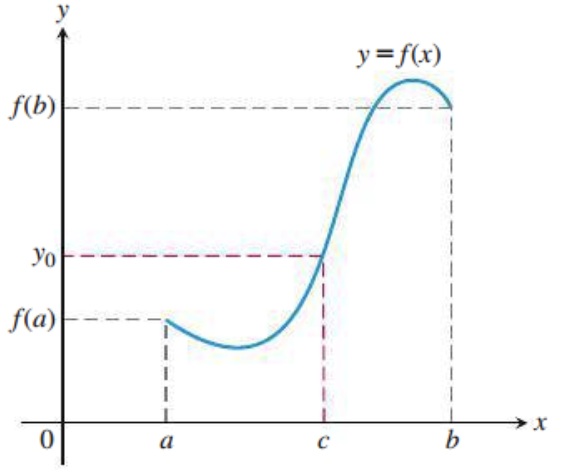
\includegraphics[width=3in]{img/IVT}
\end{center}

\begin{example}
Show that there is a real solution to the equation $\sqrt{2x+5}=4-x^2$.
\end{example}
